\newpage
\section{Probabilité}

La probabilité est une \textbf{mesure} de ces évènements.\\
On peut alors définir cette mesure particulière de manière suivante :

\begin{tcolorbox}[colback=cyan!5, colframe=cyan!70!blue, title=Définition d'une loi de probabilité]
\defn{Une \textbf{loi de probabilité $\mathbb{P}$}} est une mesure qui, à chaque évènement, associe un nombre compris entre 0 et 1.
\begin{equation}
    \mathbb{P}(\Omega) = 1\;
\end{equation}

Les lois de probabilités étant des mesures, elles doivent alors respecter la définition de la mesure (Définition \ref{def:mesure}). 
\begin{enumerate}
    \item $\mathbb{P}(\emptyset) = 0$.
    \item \textbf{Positivité} : $\mathbb{P}(A) \ge 0$.
    \item \textbf{Additivité dénombrable} : si $(A_n)_{n \ge 1}$ est une suite d’ensembles disjoints deux à deux, alors
        \[
        \mathbb{P}(A_1 \cup A_2 \cup A_3 \cup \dots) = \mathbb{P}(A_1) + \mathbb{P}(A_2) + \mathbb{P}(A_3) + \dots
    \]
    Cela signifie que la mesure de l’union d’ensembles disjoints est égale à la somme des mesures de chacun.

    
    \[
        \mathbb{P}\Big(\bigcup_{n=1}^{\infty} A_n\Big) = \sum_{n=1}^{\infty} \mathbb{P}(A_n).
    \]
En particulier, si $A\in \Omega$ et $B \in \Omega $ sont disjoints,
\[
\mathbb{P}(A \cup B) = \mathbb{P}(A) + \mathbb{P}(B)
\]
\end{enumerate}

\end{tcolorbox}

\begin{figure}[H]
    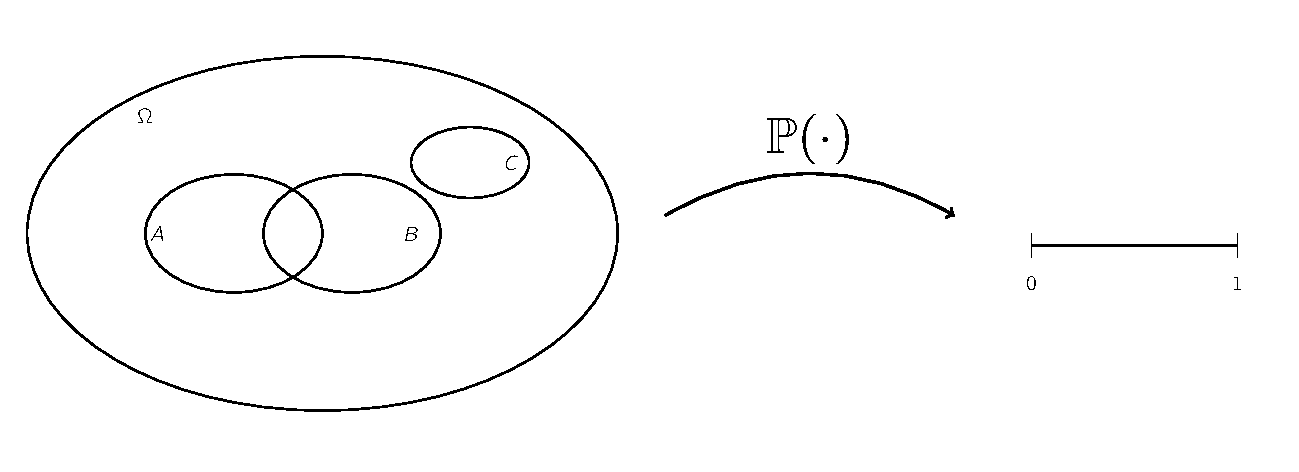
\includegraphics[scale = 0.7]{./tikz_standalone/prob_measure.pdf}
\end{figure}